	\subsection{UC 8 - Gestione alert ente}
		
		\begin{figure}[H]
			\centering
			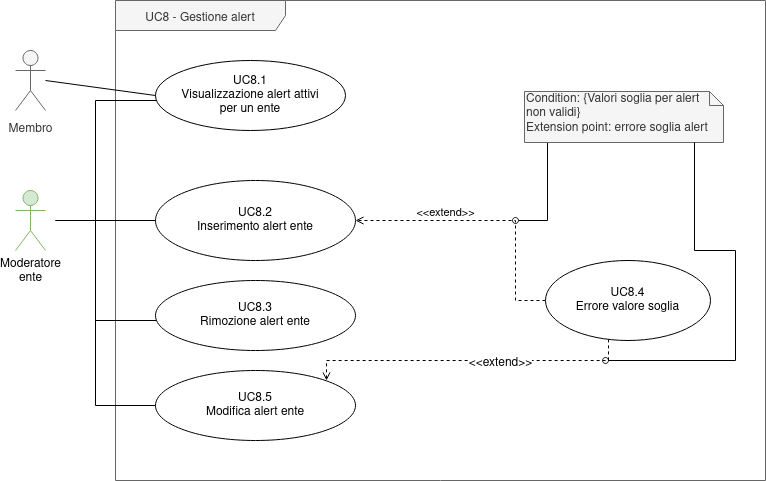
\includegraphics[scale=0.60]{res/images/uc8}
			\caption{Diagramma che descrive gli alert da abilitare per un singolo ente.}
		\end{figure}

		\begin{itemize}
			\item \textbf{Attori Primari}: Membro, Moderatore ente.
			\item \textbf{Descrizione}: L'utente gestisce gli \glock{alert} del proprio ente, impostandone le soglie oltre il quale scatenare le notifiche per gli utenti.
			\item \textbf{Precondizione}: L'utente è autenticato e naviga all'interno della gestione \glock{alert}.
			\item \textbf{Postcondizione}: L'utente ha visualizzato o gestito gli \glock{alert} del proprio ente.
			\item \textbf{Scenario Principale}:
			\begin{enumerate}
				\item{L'utente naviga all'interno della gestione \glock{alert} del proprio ente;}
				\item{L'utente ha visualizzato o gestito gli \glock{alert} del proprio ente.}
			\end{enumerate}	
		\end{itemize}
			
			\subsubsection{UC 8.1 - Visualizzazione alert ente}
			\begin{itemize}
				\item \textbf{Attori Primari}: Membro, Moderatore ente.
				\item \textbf{Descrizione}: L'utente può visualizzare gli \glock{alert} appartenenti al proprio ente.
				\item \textbf{Precondizione}: L'utente naviga all'interno della gestione \glock{alert}.
				\item \textbf{Postcondizione}: L'utente ha visualizzato la lista degli \glock{alert} del proprio ente.
				\item \textbf{Scenario Principale}:
				\begin{enumerate}
					\item{L'utente visualizza la lista degli \glock{alert} del proprio ente.}
				\end{enumerate}	
			\end{itemize}
			
			\subsubsection{UC 8.2 - Inserimento alert ente}
			\begin{itemize}
				\item \textbf{Attori Primari}: Moderatore ente.
				\item \textbf{Descrizione}: L'utente può inserire un nuovo \glock{alert} per il proprio ente.
				\item \textbf{Precondizione}: L'utente naviga all'interno della gestione \glock{alert}.
				\item \textbf{Postcondizione}: L'utente ha inserito un nuovo \glock{alert} per gli utenti appartenenti al proprio ente.
				\item \textbf{Scenario Principale}:
				\begin{enumerate}
					\item{L'utente compila i campi con i dati dell'\glock{alert} da inserire;}
					\item L'utente seleziona un sensore tra quelli disponibile su cui eseguire il controllo (UC 8.2.1);
					\item L'utente inserisce una soglia da controllare per il sensore (UC 8.2.2);
					\item{L'utente ha inserito un nuovo \glock{alert} per gli utenti appartenenti al proprio ente.}
				\end{enumerate}
				\item \textbf{Estensioni}:
				\begin{itemize}
					\item L'utente inserisce dei valori soglia non validi (UC 8.4).
				\end{itemize}		
			\end{itemize}
			
				\paragraph{UC 8.2.1 - Selezione sensore per nuovo alert}
				\begin{itemize}
					\item \textbf{Attori Primari}: Moderatore ente.
					\item \textbf{Descrizione}: L'utente compila un campo per l'inserimento di un nuovo \glock{alert} e in particolare seleziona un sensore su cui eseguire il controllo.
					\item \textbf{Precondizione}: L'utente sta inserendo i dati per un nuovo \glock{alert}.
					\item \textbf{Postcondizione}: L'utente ha compilato il campo richiesto.
					\item \textbf{Scenario Principale}:
					\begin{enumerate}
						\item{L'utente seleziona il sensore disponibile da verificare tra un elenco di quelli disponibili.}
					\end{enumerate}	
				\end{itemize}

				\paragraph{UC 8.2.2 - Inserimento soglia per nuovo alert}
				\begin{itemize}
					\item \textbf{Attori Primari}: Moderatore ente.
					\item \textbf{Descrizione}: L'utente compila un campo per l'inserimento di un nuovo \glock{alert} e in particolare seleziona la soglia da controllare.
					\item \textbf{Precondizione}: L'utente sta inserendo i dati per un nuovo \glock{alert}.
					\item \textbf{Postcondizione}: L'utente ha compilato il campo richiesto.
					\item \textbf{Scenario Principale}:
					\begin{enumerate}
						\item{L'utente inserisce la soglia del sensore da verificare.}
					\end{enumerate}	
				\end{itemize}

			\subsubsection{UC 8.3 - Rimozione alert ente}
			\begin{itemize}
				\item \textbf{Attori Primari}: Moderatore ente.
				\item \textbf{Descrizione}: L'utente può rimuovere un \glock{alert} selezionandolo dalla lista degli \glock{alert} attivi del proprio ente.
				\item \textbf{Precondizione}: L'utente naviga all'interno della gestione \glock{alert} e ha disponibile almeno un alert.
				\item \textbf{Postcondizione}: L'utente ha rimosso l'\glock{alert} selezionato del proprio ente dal sistema.
				\item \textbf{Scenario Principale}:
				\begin{enumerate}
					\item{L'utente seleziona un \glock{alert} dalla lista degli \glock{alert} del proprio ente e lo rimuove;}
					\item{L'utente non visualizza più l'\glock{alert} selezionato.}
				\end{enumerate}	
			\end{itemize}

			\subsubsection{UC 8.4 - Errore valore soglia}
			\begin{itemize}
				\item \textbf{Attori Primari}: Moderatore ente.
				\item \textbf{Descrizione}: Dopo aver premuto il bottone per confermare i campi inseriti, viene visualizzato il messaggio di errore che segnala un valore soglia non valido.
				\item \textbf{Precondizione}: L'utente ha inserito i campi richiesti e il sistema sta elaborando la richiesta.
				\item \textbf{Postcondizione}: Visualizzazione messaggio di errore specifico.
				\item \textbf{Scenario Principale}:
				\begin{enumerate}
					\item{Il sistema elabora la richiesta;}
					\item{Viene visualizzato il messaggio di errore che spiega che il valore soglia inserito per un \glock{alert} non è valido. }
				\end{enumerate}
			\end{itemize}
			
			\subsubsection{UC 8.5 - Modifica alert ente}
			\begin{itemize}
				\item \textbf{Attori Primari}: Moderatore ente.
				\item \textbf{Descrizione}: L'utente può modificare \glock{alert} esistente per il proprio ente.
				\item \textbf{Precondizione}: L'utente naviga all'interno della gestione \glock{alert}.
				\item \textbf{Postcondizione}: L'utente ha inserito un nuovo \glock{alert} per gli utenti appartenenti al proprio ente.
				\item \textbf{Scenario Principale}:
				\begin{enumerate}
					\item{L'utente compila i campi con i dati dell'\glock{alert} da inserire;}
					\item L'utente modifica la soglia da controllare per il sensore (UC 8.5.1);
					\item{L'utente ha inserito un nuovo \glock{alert} per gli utenti appartenenti al proprio ente.}
				\end{enumerate}
				\item \textbf{Estensioni}:
				\begin{itemize}
					\item L'utente inserisce dei valori soglia non validi (UC 8.4).
				\end{itemize}		
			\end{itemize}

				\paragraph{UC 8.5.1 - Modifica soglia per alert}
				\begin{itemize}
					\item \textbf{Attori Primari}: Moderatore ente.
					\item \textbf{Descrizione}: L'utente compila un campo per la modifica di un \glock{alert} e in particolare inserisce la soglia da controllare.
					\item \textbf{Precondizione}: L'utente sta inserendo i dati per modificare un \glock{alert}.
					\item \textbf{Postcondizione}: L'utente ha compilato il campo richiesto.
					\item \textbf{Scenario Principale}:
					\begin{enumerate}
						\item{L'utente inserisce la soglia del sensore da verificare.}
					\end{enumerate}	
				\end{itemize}